%\documentclass[a4,semhelv,landscape]{seminar}
\documentclass[landscape]{slides}
%\documentclass[pdf, default, slideBW, nocolorBG]{prosper}
\usepackage[left=0.2cm,top=0.2cm,right=0.2cm,bottom=0.2cm,nohead,nofoot]{geometry}
%\def\everyslide{\sffamily}
%\usepackage{fullpage}
\usepackage{graphicx}
\usepackage[usenames]{color}
%\usepackage{color}
\usepackage{verbatim}
\usepackage{nopageno}
\usepackage{setspace}
%\usepackage{times}
% define some nice colors
\definecolor{myred}{rgb}{0.6,0,0}
\definecolor{myblue}{rgb}{0,0.2,0.4}
\definecolor{mygreen}{rgb}{0,0.5,0.0}
\definecolor{mypurple}{cmyk}{0.5,1.0,0.0,0.0}
%\color{myblue}

\begin{document}
%%%%%%%%%%%%%%%%%%%%%%%%%%%%%%%%%%%%%%%%%%%%%%%%%%%%%%%%%%%%%%%%%%%%
%Slide 0 - title
\begin{slide}
\begin{center}
\large{\textbf{Reference-guided annotation of viral genomes}}

\normalsize

Eric Nawrocki \\

\medskip

\medskip

\medskip

\medskip

\medskip

\small
\begin{tabular}{c}
Alejandro Sch\"{a}ffer's group \\
\\
National Center for Biotechnology Information\\
National Institutes of Health\\
\\
\end{tabular}

\vspace{0.1in}


\includegraphics[width=2.5in]{figs/ncbi-logo}

\end{center}
\end{slide}
%%%%%%%%%%%%%%%%%%%%%%%%%%%%%%%%%%%%%%%%%%%%%%%%%%%%%%%%%%%%%%%%%%%%%%
\begin{slide}
\begin{center}

\textbf{Most prevalent viral genomes in GenBank\footnote{Influenza is omitted.}}

\tiny
\begin{tabular}{r|l|r|l|l|l|r|r}
       &                    &              &                &          &        &       & \#mature \\ 
  rank & species            &       \#seqs & family         & type     & host   & \#cds & peptides \\ \hline
       &                    &              &                &          &        &       &          \\ 
     1 & Hepatitis B        &         7061 & Hepadnaviridae & dsDNA-RT & humans &     7 &       -  \\
       &                    &              &                &          &        &       &          \\ 
     2 & Dengue             &         3875 & Flaviviridae   & (+)ssRNA & humans &     1 &      14  \\
       &                    &              &                &          &        &       &          \\ 
     3 & West Nile          &        2218  & Flaviviridae   & (+)ssRNA & humans &     3 &      16  \\
       &                    &              &                &          &        &       &          \\ 
     4 & Rotavirus          &      22536*  & Reoviridae     & dsRNA    & humans &    12 &       -  \\
       &                    &              &                &          &        &       &          \\ 
     5 & HIV-1              &        2132  & Retroviridae   & ssRNA-RT & humans &    10 &      14  \\
       &                    &              &                &          &        &       &          \\ 
     6 & Porcine circovirus &        1559  & Circoviridae   & ssDNA    & pigs   &     3 &       -  \\
       &                    &              &                &          &        &       &          \\ 
     7 & Hepatitis C        &        1457  & Flaviviridae   & (+)ssRNA & humans &     2 &      10  \\
       &                    &              &                &          &        &       &          \\ 
     8 & Ebola              &        1105  & Flaviviridae   & (+)ssRNA & humans &     9 &       -  \\
       &                    &              &                &          &        &       &          \\ 
     9 & Enterovirus A      &         932  & Picarnoviridae & (+)ssRNA & humans &     1 &      11  \\
       &                    &              &                &          &        &       &          \\ 
    10 & RSV                &         623  & Paramyxoviridae& (-)ssRNA & humans &    11 &       -  \\
       &                    &              &                &          &        &       &          \\ 
    11 & Enterovirus C (Polio) &      618  & Picarnoviridae & (+)ssRNA & humans &     1 &      13  \\
       &                    &              &                &          &        &       &          \\ 
    12 & JC polyomavirus    &          598 & Polyomaviridae & dsDNA    & humans &     6 &       -  \\
       &                    &              &                &          &        &       &          \\ 
    13 & PRRSV              &          520 & Arteriviridae  & (+)ssRNA & pigs   &    11 &      13  \\ %# 15 mat_peptide segments, 13 mat_peptides 
       &                    &              &                &          &        &       &          \\ 
    14 & Maize streak virus &          508 & Geminiviridae  & ssDNA    & plants &     4 &      -   \\
       &                    &              &                &          &        &       &          \\ 
    15 & Norwalk virus      &          491 &  Calciviridae  & (+)ssRNA & humans &     3 &       6  \\ 
\end{tabular}

% SAME TABLE, WITH EXON COUNTS
%\tiny
%\begin{tabular}{r|l|r|l|l|l|r|r|r}
%       &                    &              &                &          &        &       &        & mature   \\ 
%   rank& species            &     \# seqs & family         & type     & host   & \#cds &\#exons & peptides \\ \hline
%     1 & Hepatitis B        &        7061 & Hepadnaviridae  & dsDNA-RT & humans &     7 &      7 &       -  \\
%     2 & Dengue             &        3875 & Flaviviridae    & (+)ssRNA & humans &     1 &      1 &      14  \\
%     3 & Rotavirus          &      22536* & Reoviridae      & dsRNA    & humans &    12 &      ? &       -  \\
%     4 & HIV-1              &        2132 & Retroviridae    & ssRNA-RT & humans &    10 &     14 &      14  \\
%     5 & Porcine circovirus &        1559 & Circoviridae    & ssDNA    & pigs   &     3 &      3 &       -  \\
%     6 & Hepatitis C        &        1457 & Flaviviridae    & (+)ssRNA & humans &     2 &      3 &      10  \\
%     7 & West Nile          &       2218* & Flaviviridae    & (+)ssRNA & humans &     3 &      5 &      16  \\
%     8 & Ebola              &        1105 & Flaviviridae    & (+)ssRNA & humans &     9 &     11 &       -  \\
%     9 & Enterovirus A      &         932 & Picarnoviridae  & (+)ssRNA & humans &     1 &      1 &      11  \\
%    10 & RSV                &         623 & Paramyxoviridae & (-)ssRNA & humans &    11 &     11 &       -  \\
%    11 & Enterovirus C (Polio) &      618 & Picarnoviridae  & (+)ssRNA & humans &     1 &      1 &      13  \\
%    12 & JC polyomavirus   &          598 & Polyomaviridae  & dsDNA    & humans &     6 &      7 &       -  \\
%    13 & PRRSV             &          520 & Arteriviridae   & (+)ssRNA & pigs   &    11 &     13 &  13(15)  \\ %# 15 mat_peptide segments, 13 mat_peptides 
%    14 & Maize streak virus&          508 & Geminiviridae   & ssDNA    & plants &     4 &      5 &      -   \\
%    15 & Norwalk virus     &          491 &  Calciviridae   & (+)ssRNA & humans &     3 &      3 &      6   \\ 
%\end{tabular}

\end{center}
\end{slide}
%%%%%%%%%%%%%%%%%%%%%%%%%%%%%%%%%%%%%%%%%%%%%%%%%%%%%%%%%%%%%%%%%%%%%%


\begin{slide}
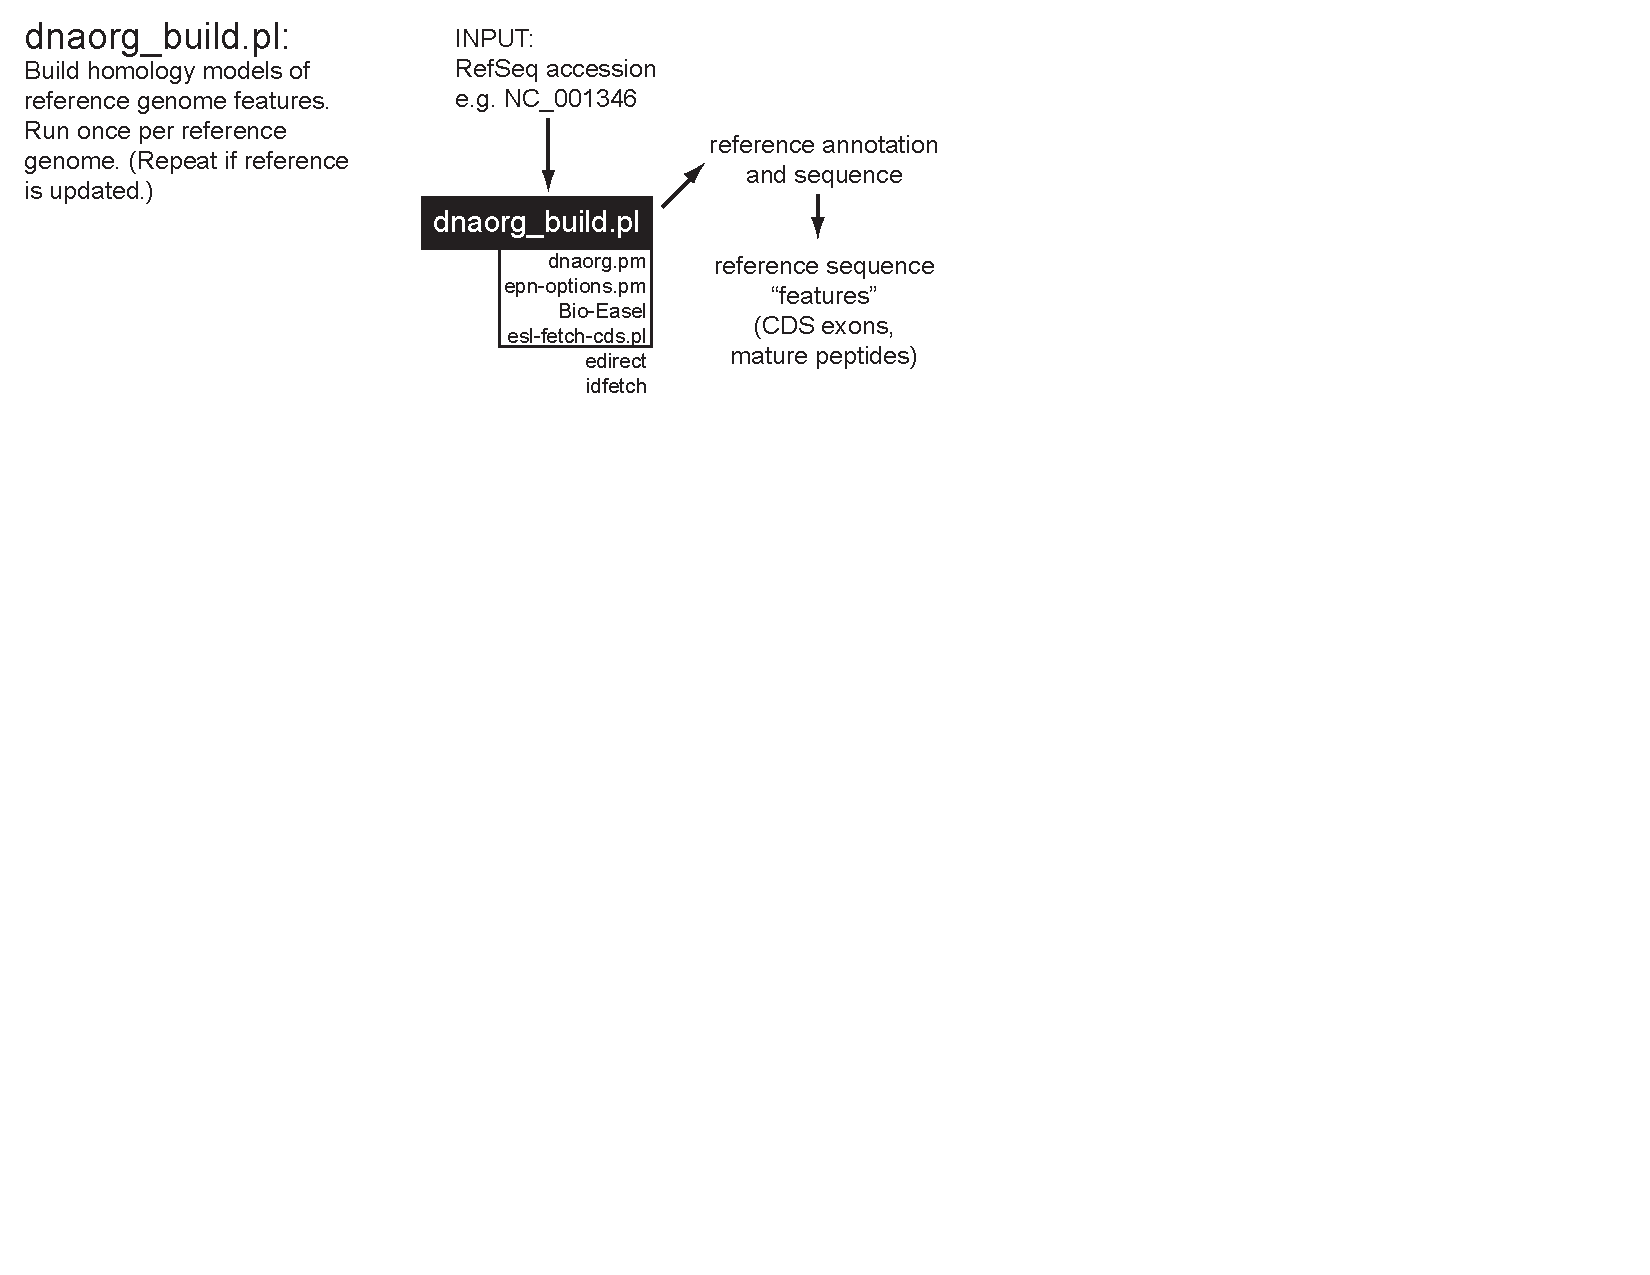
\includegraphics[width=10in]{figs/dnaorg-scripts-build1}
\vfill
\end{slide}
%%%%%%%%%%%%%%%%%%%%%%%%%%%%%%%%%%%%%%%%%%%%%%%%%%%%%%%%%%%%%%%%%%%%%%
\begin{slide}
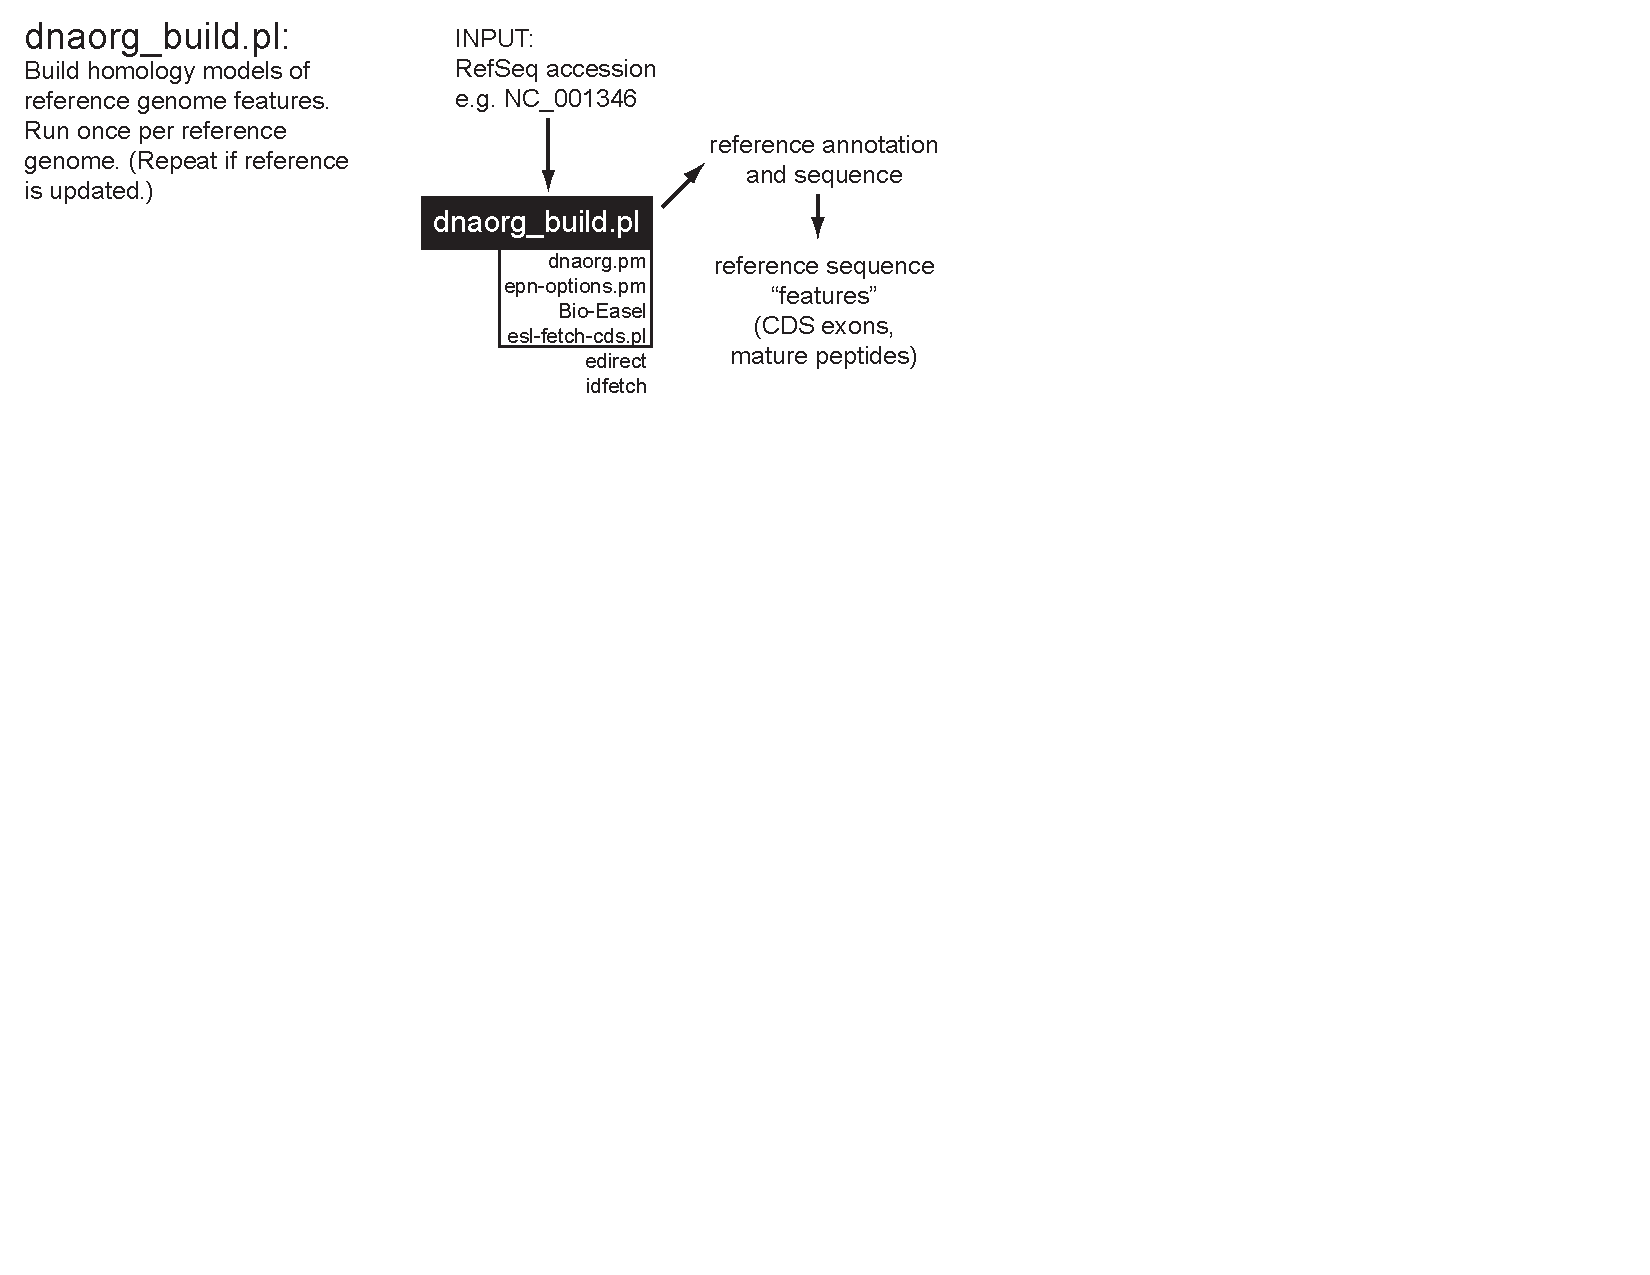
\includegraphics[width=10in]{figs/dnaorg-scripts-build1}
\vfill
\end{slide}
%%%%%%%%%%%%%%%%%%%%%%%%%%%%%%%%%%%%%%%%%%%%%%%%%%%%%%%%%%%%%%%%%%%%%%
\begin{slide}
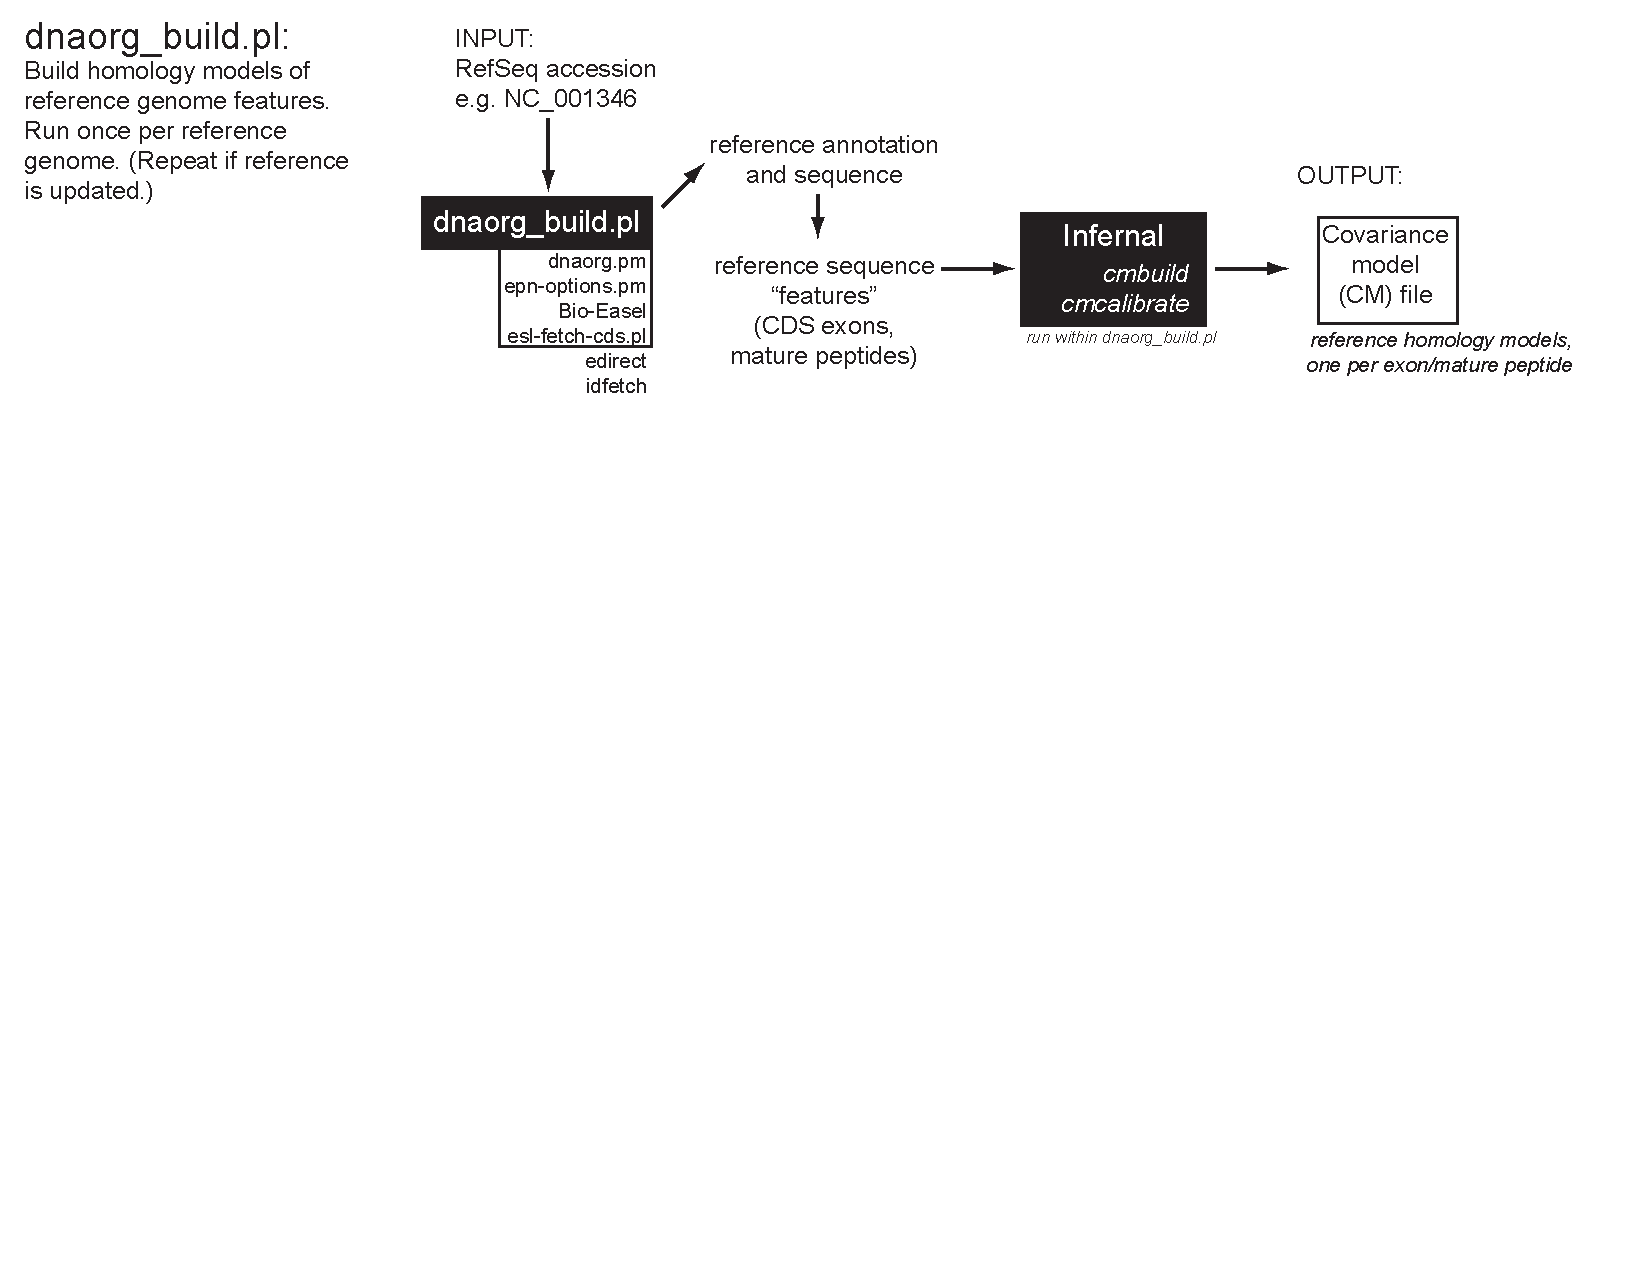
\includegraphics[width=10in]{figs/dnaorg-scripts-build2}
\vfill
\end{slide}
%%%%%%%%%%%%%%%%%%%%%%%%%%%%%%%%%%%%%%%%%%%%%%%%%%%%%%%%%%%%%%%%%%%%%%
\begin{slide}
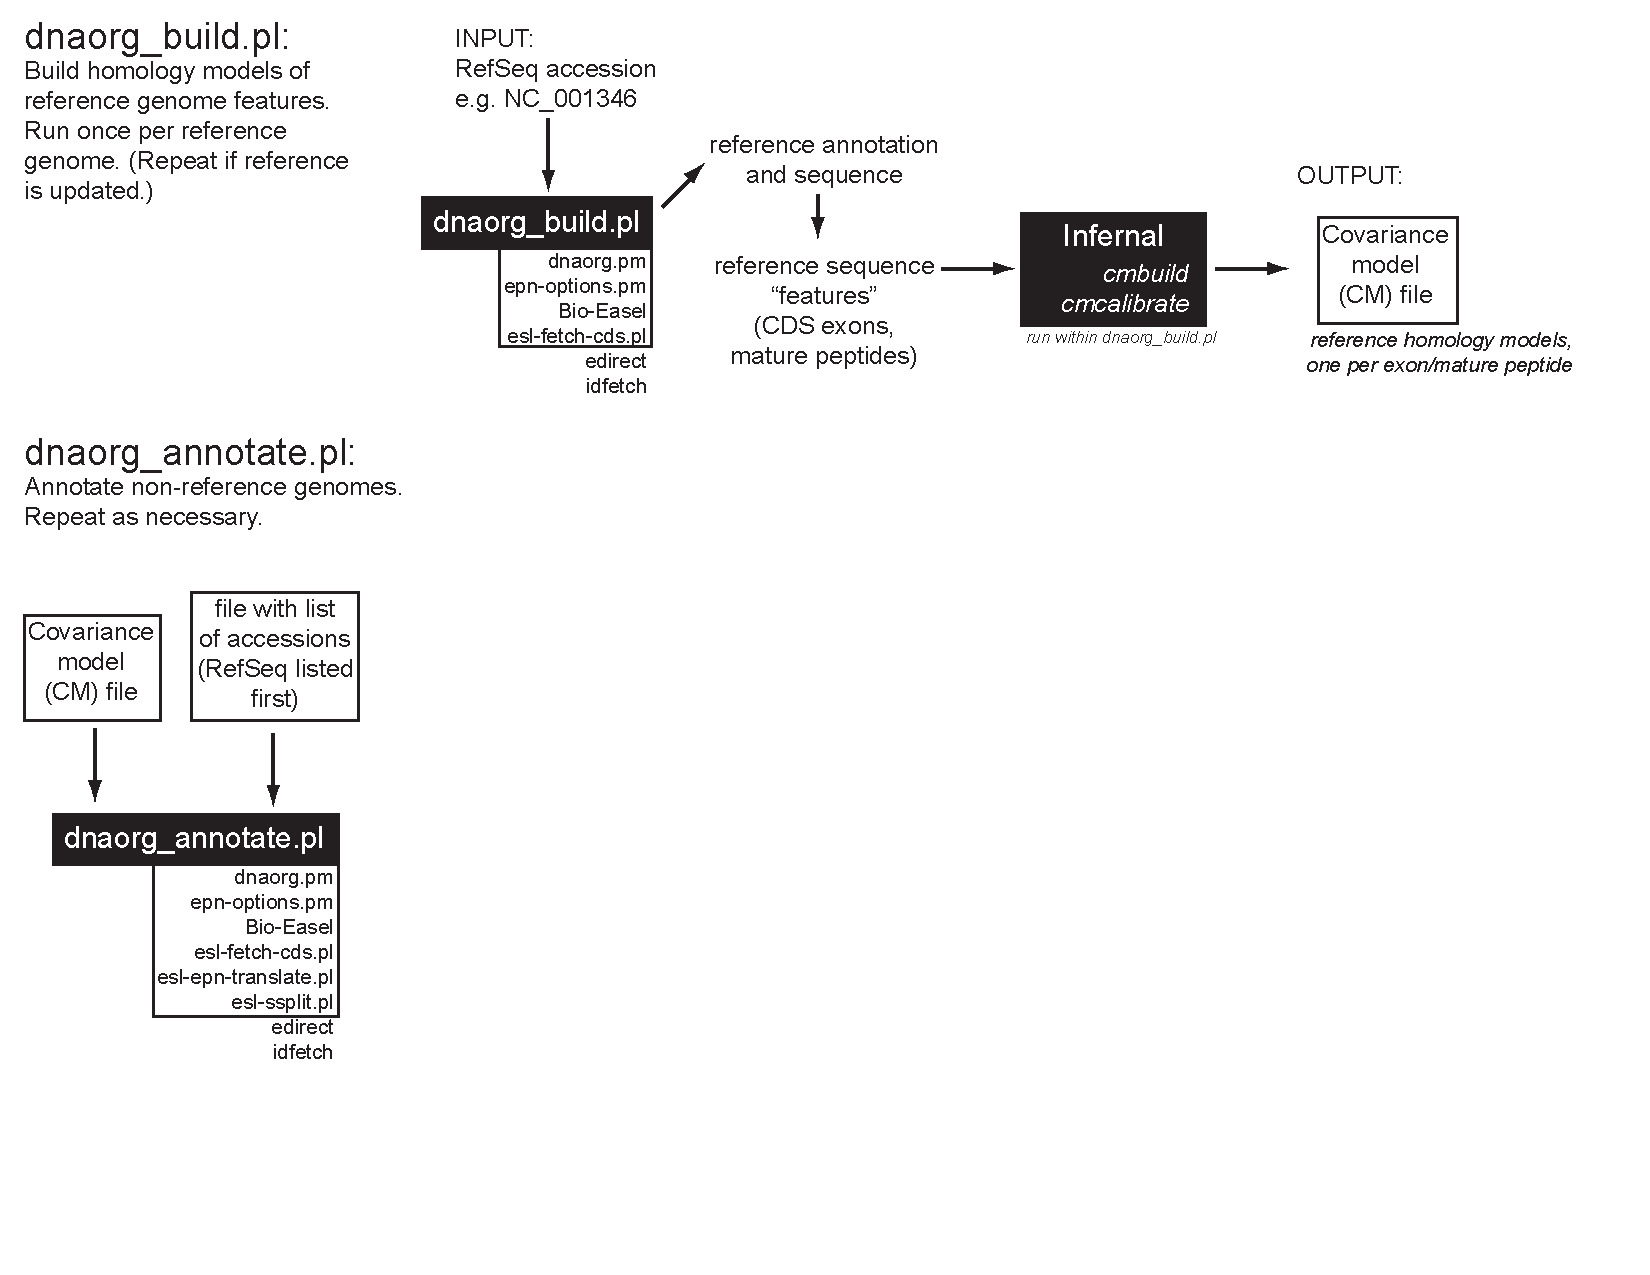
\includegraphics[width=10in]{figs/dnaorg-scripts-annotate1}
\vfill
\end{slide}
%%%%%%%%%%%%%%%%%%%%%%%%%%%%%%%%%%%%%%%%%%%%%%%%%%%%%%%%%%%%%%%%%%%%%%
\begin{slide}
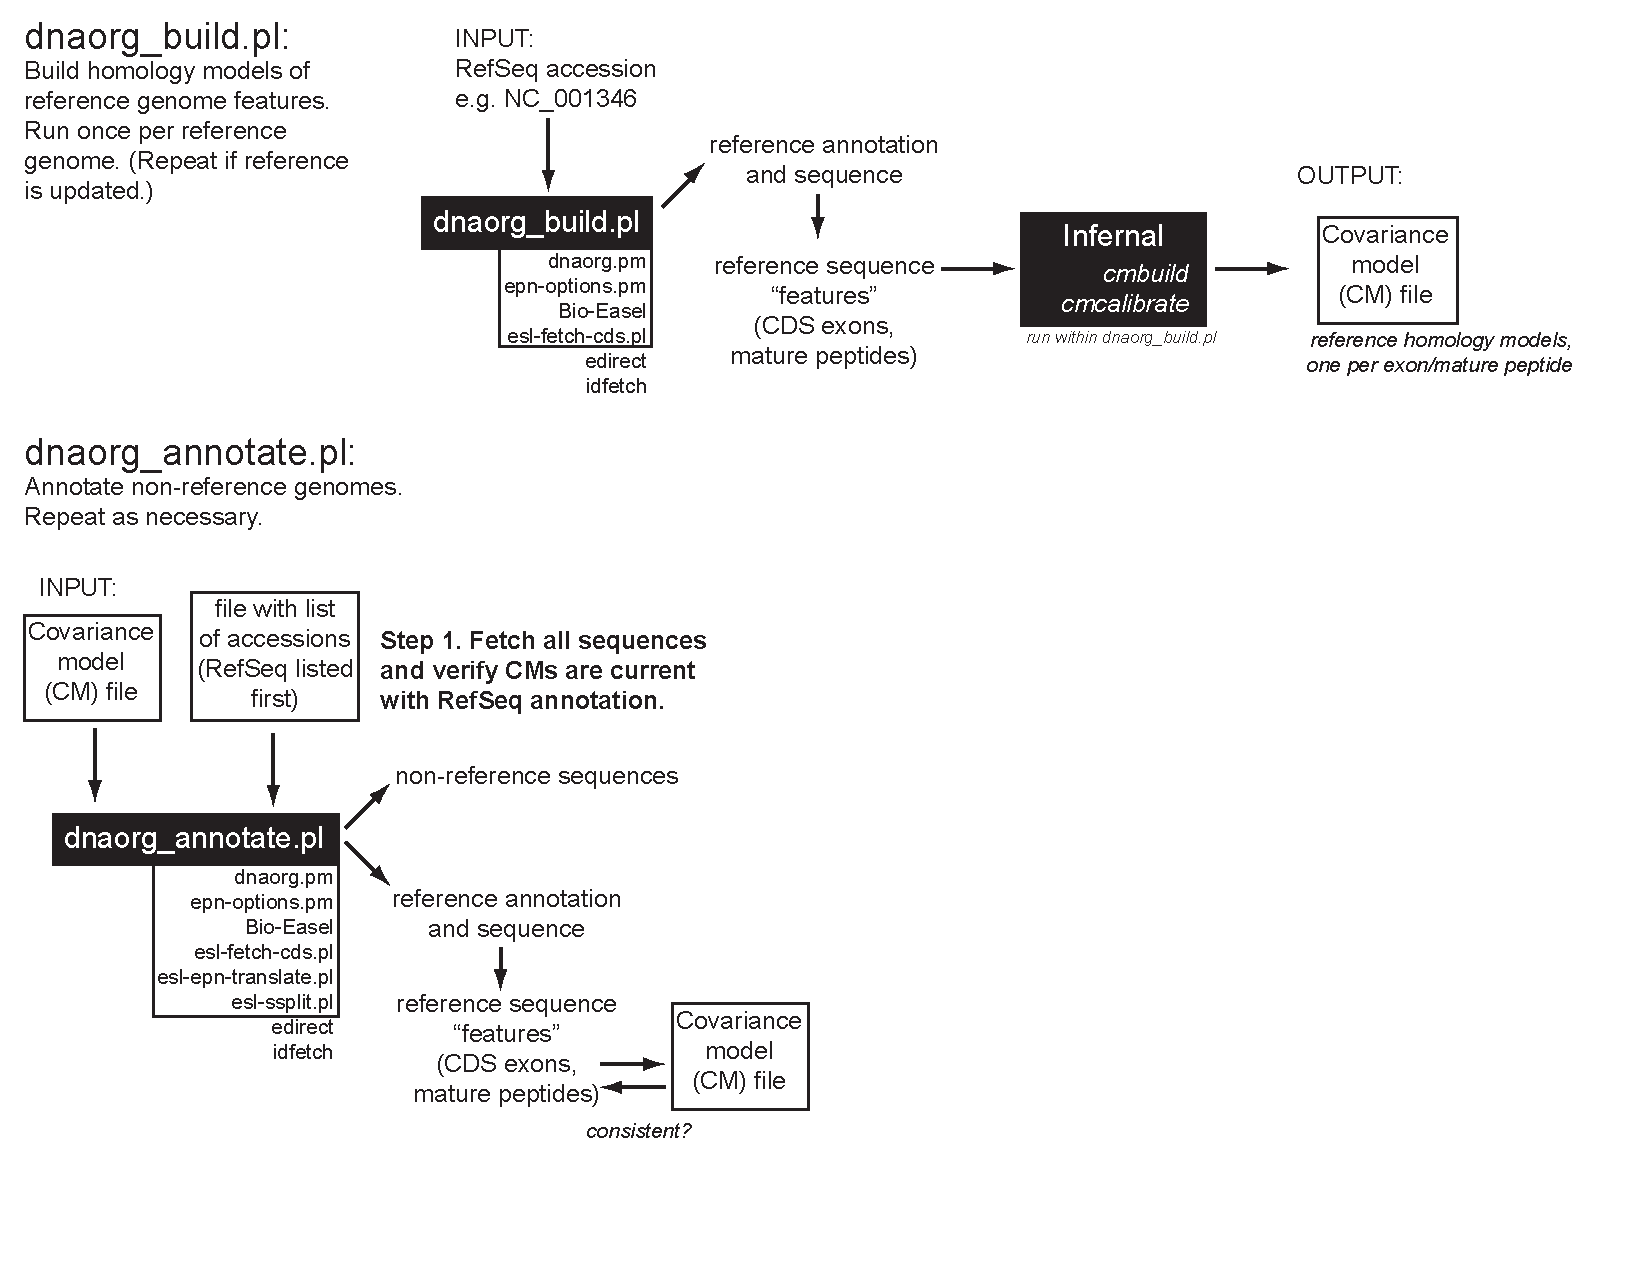
\includegraphics[width=10in]{figs/dnaorg-scripts-annotate2}
\vfill
\end{slide}
%%%%%%%%%%%%%%%%%%%%%%%%%%%%%%%%%%%%%%%%%%%%%%%%%%%%%%%%%%%%%%%%%%%%%%
\begin{slide}
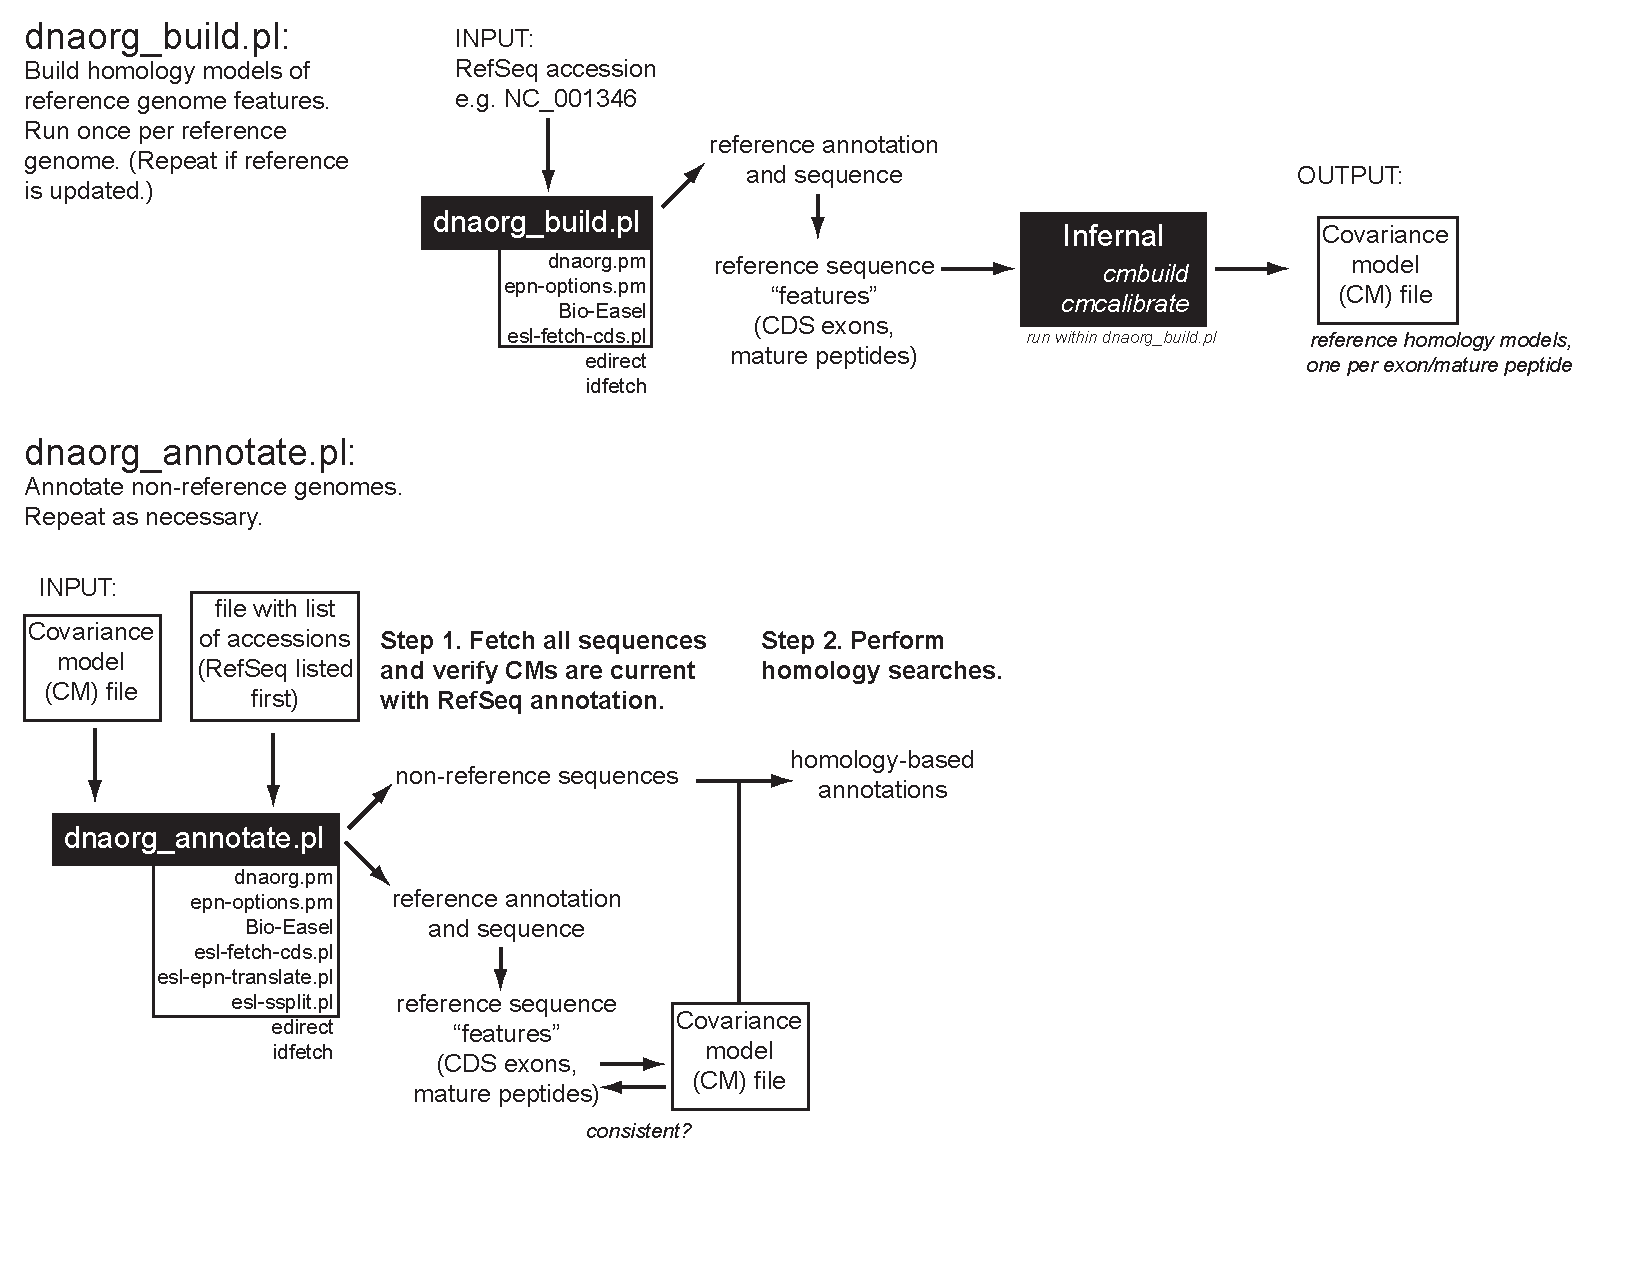
\includegraphics[width=10in]{figs/dnaorg-scripts-annotate3}
\vfill
\end{slide}
%%%%%%%%%%%%%%%%%%%%%%%%%%%%%%%%%%%%%%%%%%%%%%%%%%%%%%%%%%%%%%%%%%%%%%
\begin{slide}
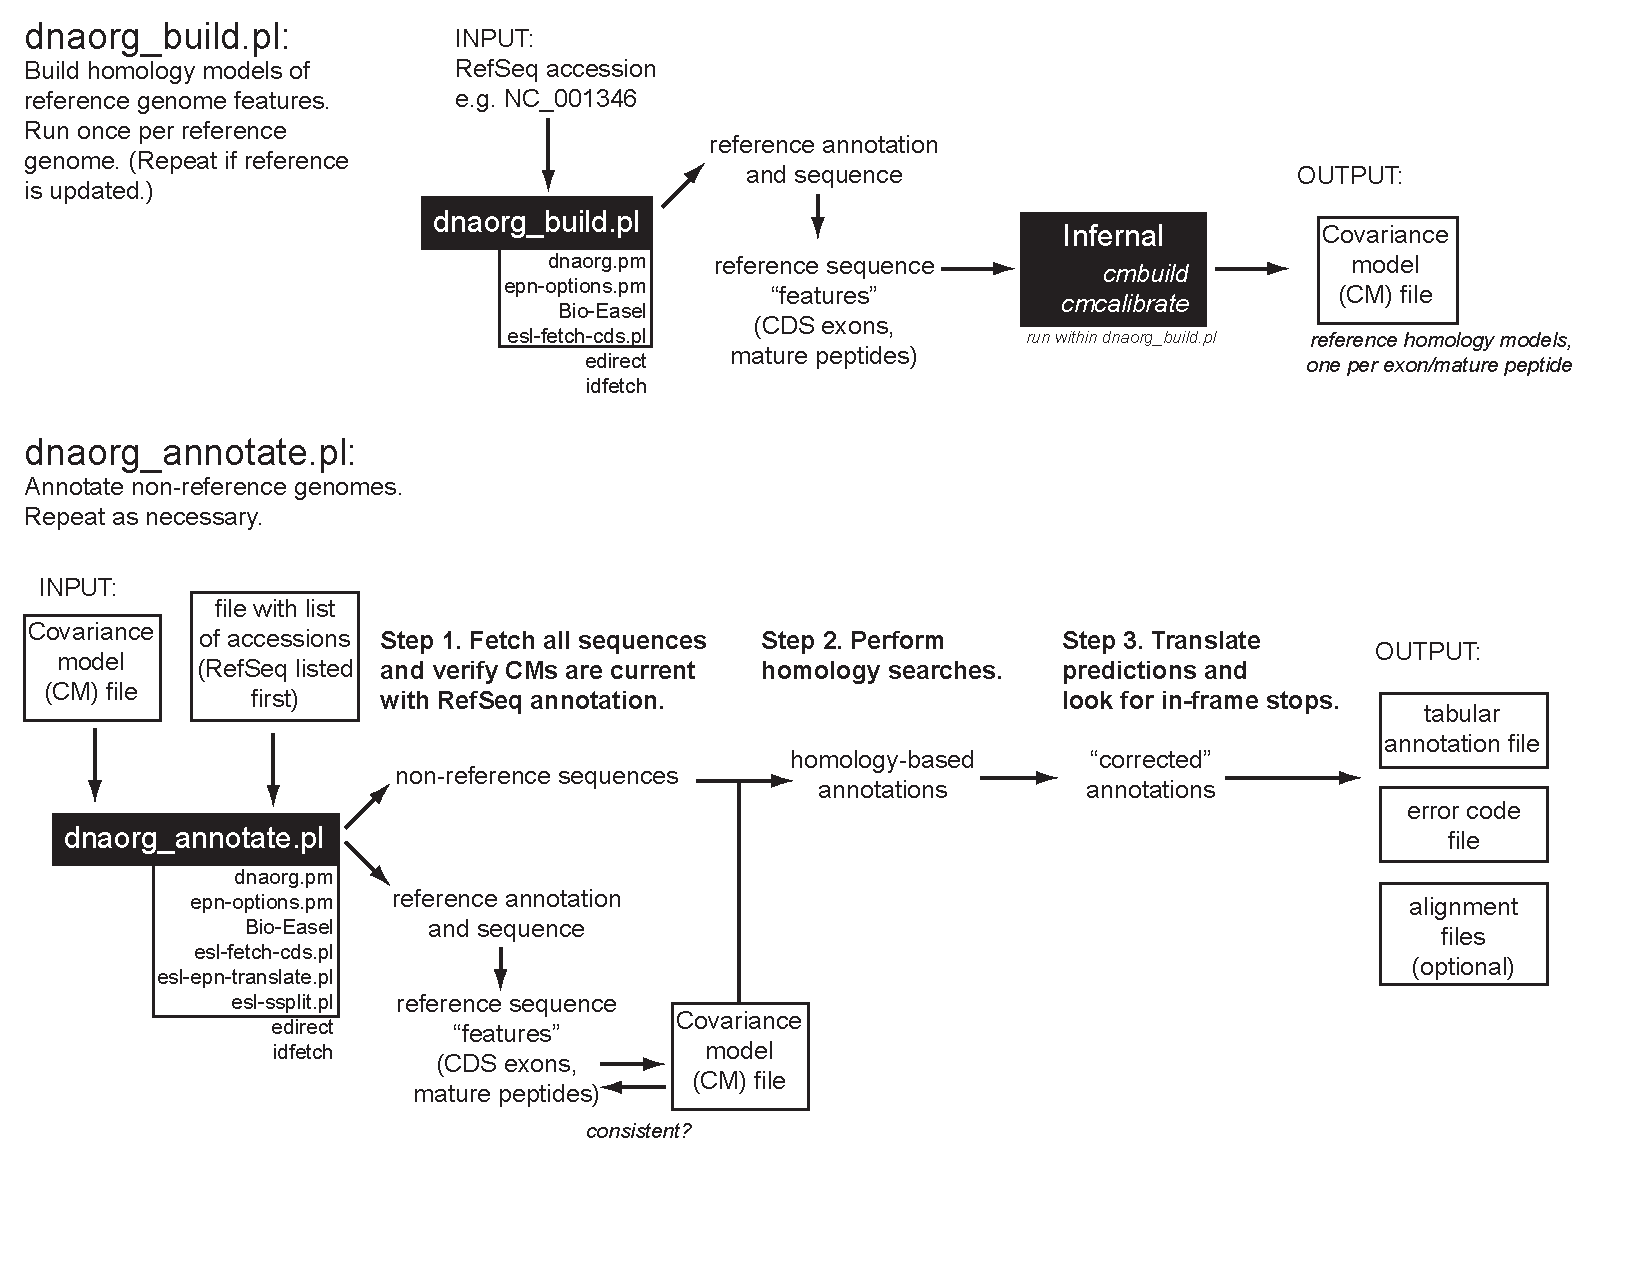
\includegraphics[width=10in]{figs/dnaorg-scripts-annotate4}
\vfill
\end{slide}
%%%%%%%%%%%%%%%%%%%%%%%%%%%%%%%%%%%%%%%%%%%%%%%%%%%%%%%%%%%%%%%%%%%%%%
% 
% Pilot species:
%%%%%%%%%%%%%%%%%%%%%%%%%%%%%%%%%%%%%%%%%%%%%%%%%%%%%%%%%%%%%%%%%%%%%%
\begin{slide}
\textbf{West Nile virus}

\begin{center}
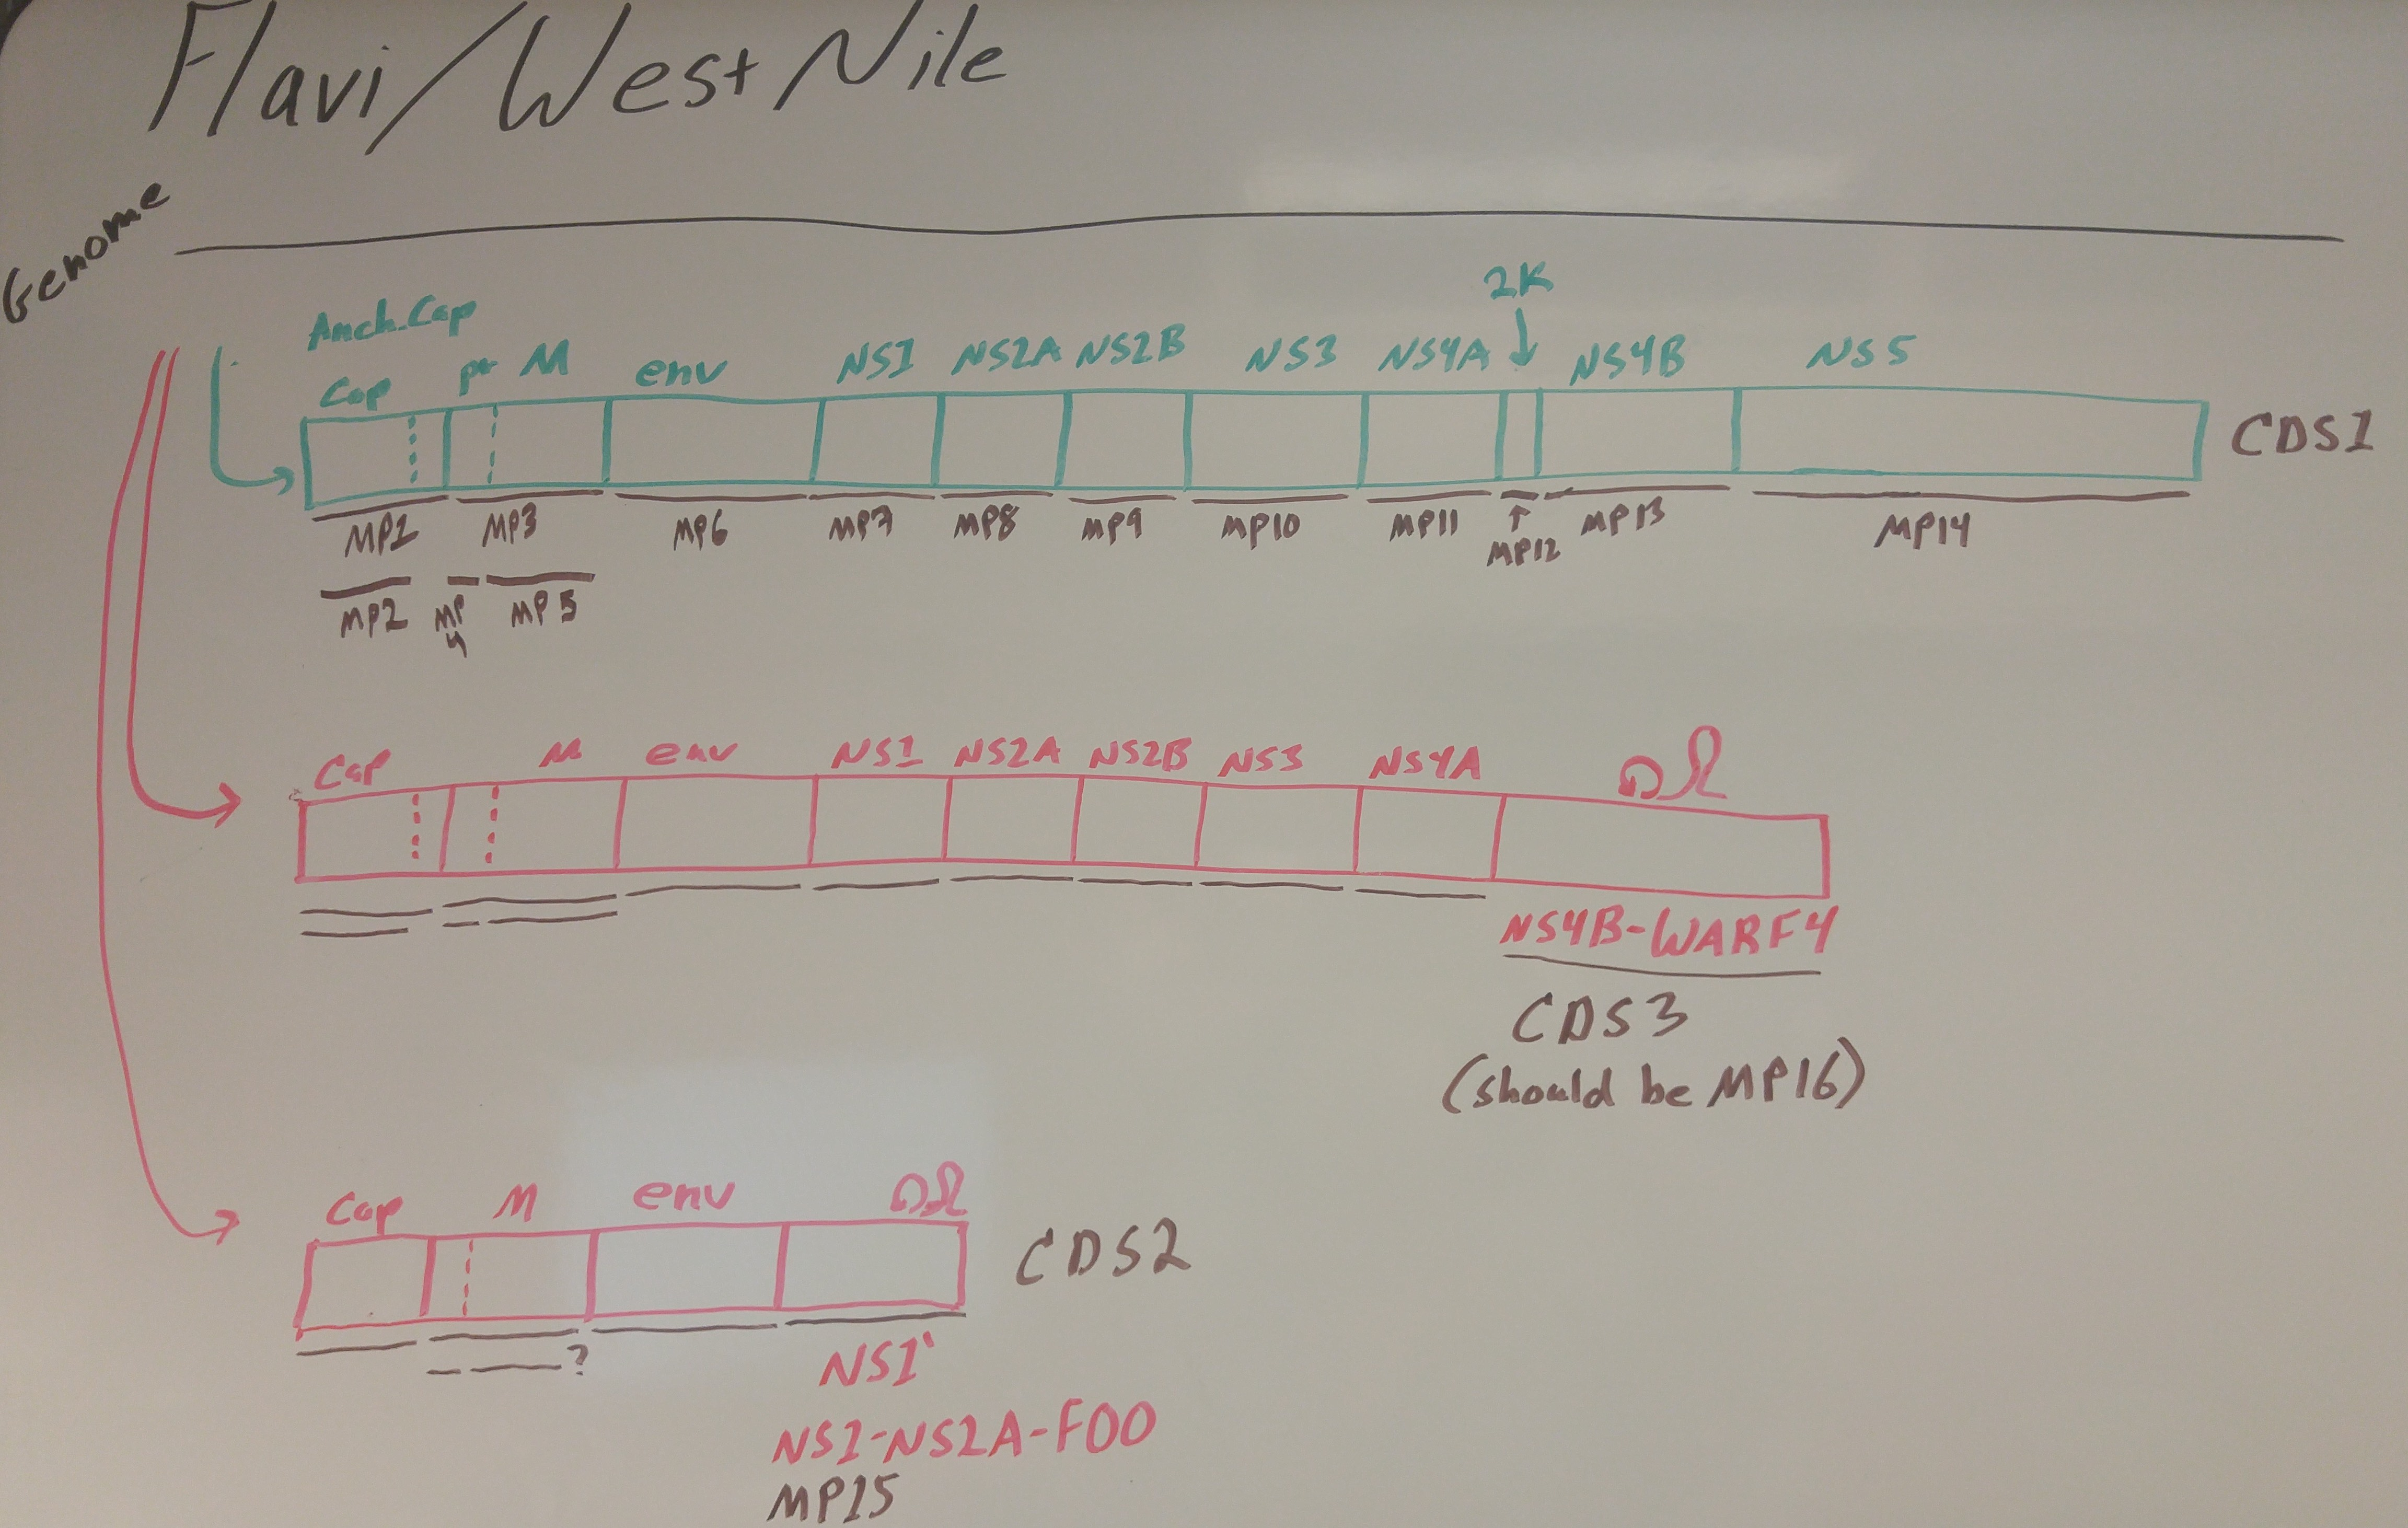
\includegraphics[width=8in]{figs/flavi-wnv-eneida}
\end{center}
\vfill
\end{slide}
%%%%%%%%%%%%%%%%%%%%%%%%%%%%%%%%%%%%%%%%%%%%%%%%%%%%%%%%%%%%%%%%%%%%%%
\end{document}
